\documentclass[final,hyperref={pdfpagelabels=false},aspectratio=169,t]{beamer}
\mode<presentation> {
  \usecolortheme{rose}
  \setbeamertemplate{footline}[page number] 
  \setbeamertemplate{navigation symbols}{} 
  \usefonttheme{professionalfonts}}


\usepackage{graphicx} % Allows including images
\usepackage{booktabs} % Allows the use of \toprule, \midrule and \bottomrule in tables

\usepackage{geometry}
\usepackage{xspace}

\usepackage[utf8]{inputenc}
\usepackage{default}
\usepackage{amsmath}
\usepackage{amsfonts}
\usepackage{amssymb}
\usepackage{amsthm}
\usepackage{bm}
\usepackage{slashed}

\usepackage{tikz}

\usepackage[overlay,absolute]{textpos}
\setlength{\TPHorizModule}{1cm}
\setlength{\TPVertModule}{1cm}
\textblockorigin{10mm}{10mm}
\input{/Users/marin/tex/GA/presentations/NewCommands.tex}

\graphicspath{
  {./IMAGES/}
{/Users/marin/tex/GA/presentations/}
{/Users/marin/PhysicsTalks/PhysicsFigures/}
}

%----------------------------------------------------------------------------------------
%       TITLE PAGE
%----------------------------------------------------------------------------------------

\date{\today} % Date, can be changed to a custom date

\title{\texorpdfstring{\LARGE Central and Forward rapidity. $\eta$ meson }}
%N$^\gamma$/N$_{ch}$\\ 
%Study of Inclusive photons in RBins 

\author[A.Marin]{Ana Marin}
\institute[GSI]{\small GSI, Darmstadt, Germany}
%\today


\begin{document}
\begin{frame}

  \begin{textblock}{14}(0.0,1.0)
    \titlepage
  \end{textblock}
  

 % the logos
 \begin{textblock}{12}(0.0,5.7)
     \includegraphics[width=3cm]{GSI_Logo_cmyk}
\end{textblock}

  \begin{textblock}{12}(11.,4.7)
    \includegraphics[width=1.5cm]{2012-Jul-04-4_Color_Logo_CB}
  \end{textblock}

\end{frame}
%\end{document}

\begin{frame}
\frametitle{Simulation settings}

\begin{itemize}
\item  Full simulations of pp $\sqrt{s} =$ 14 TeV using PYTHIA 8.2  in local HD cluster  (2.2$\times$10$^6$events generated) 
\item  Analysis using MC information: \\
 Central: $|\eta| < $1.3 (\pT $ > $ 0.1 \GeVc) \\
 Forward: 1.7$ < |\eta| < $ 4 (p $ > $ 0.1 \GeVc)   
\end{itemize}
\end{frame}


\begin{frame}
\frametitle{$\eta$ meson $\rightarrow$ $\gamma \gamma$}
%\vspace*{-0.4cm}

\begin{tabular}{ccc}
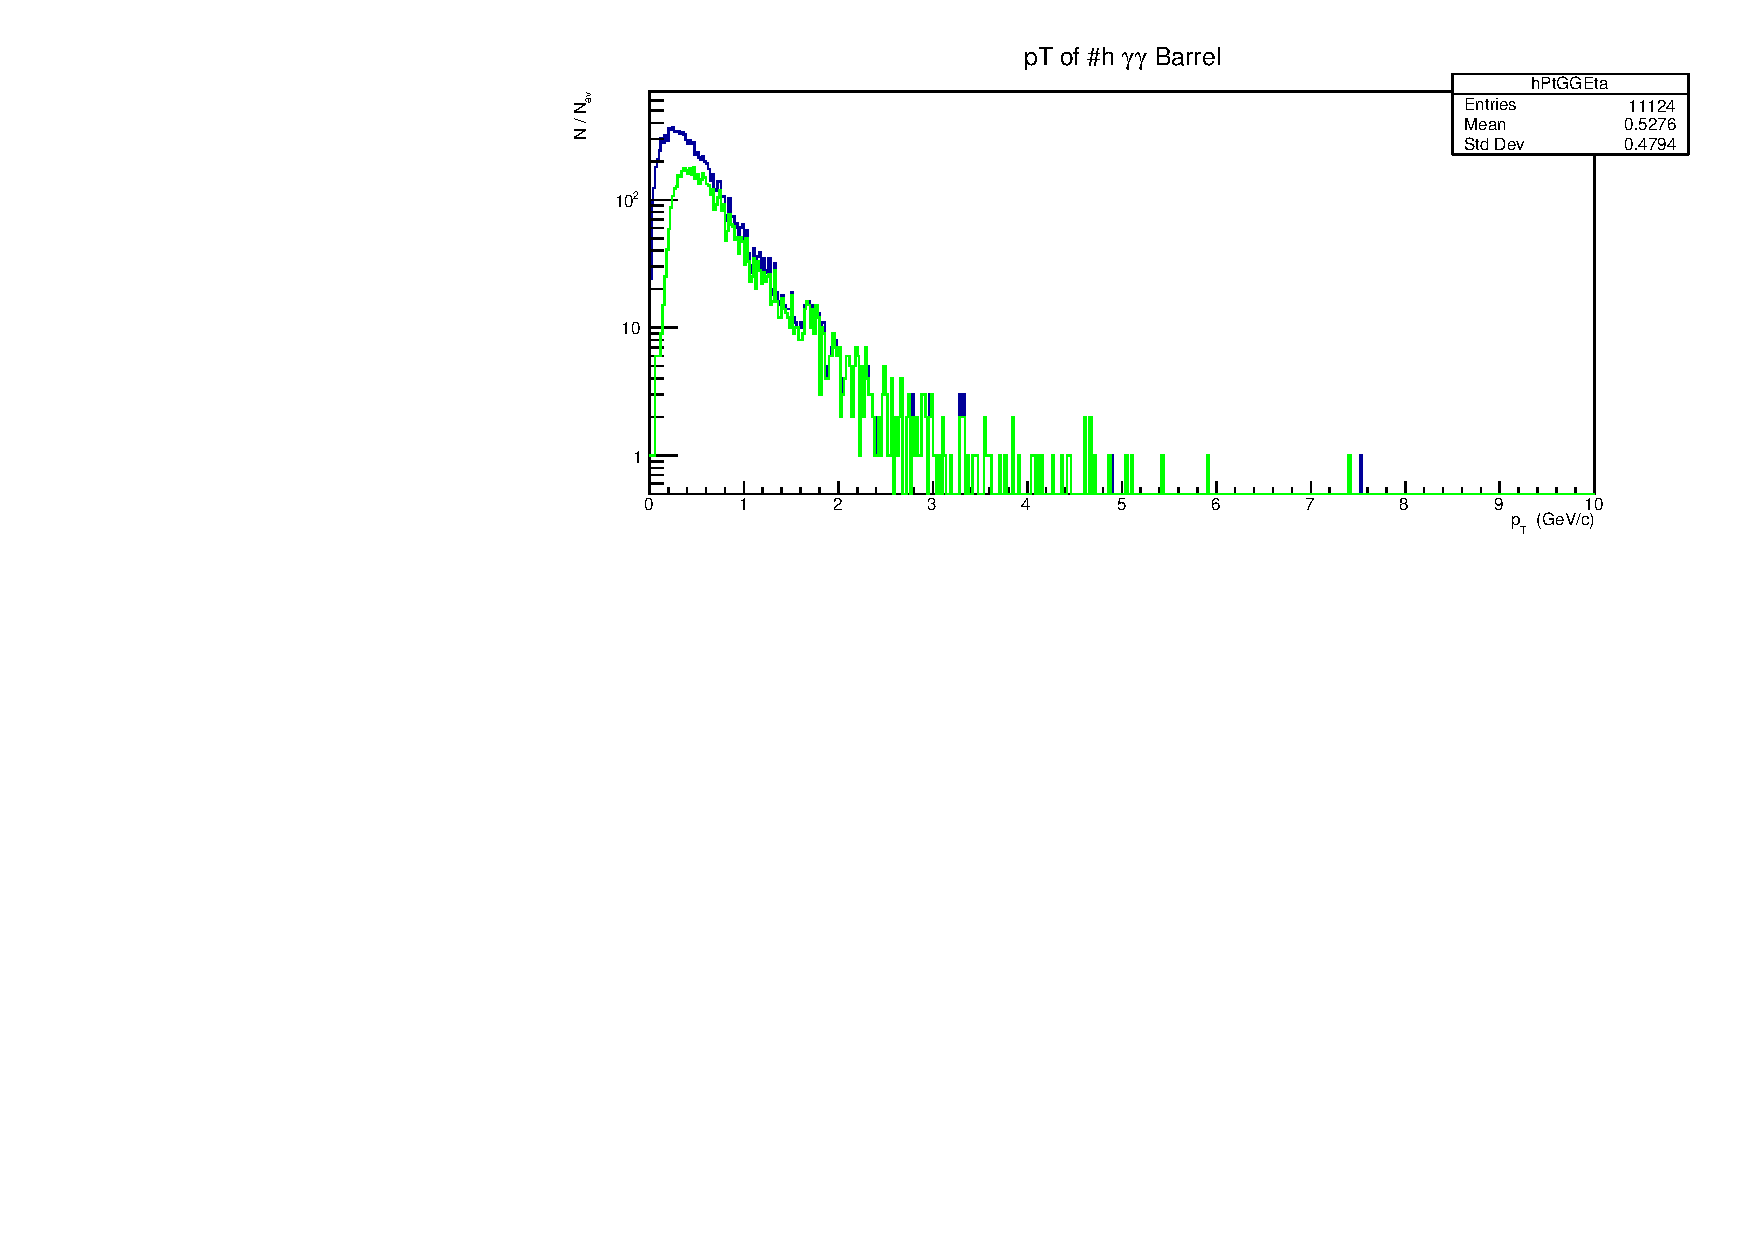
\includegraphics[width=0.32\textwidth]{/Users/marin/alice3/alice3Conversions//anaConv/EtaMeson-EtaMesonCut-Barrel.pdf}&
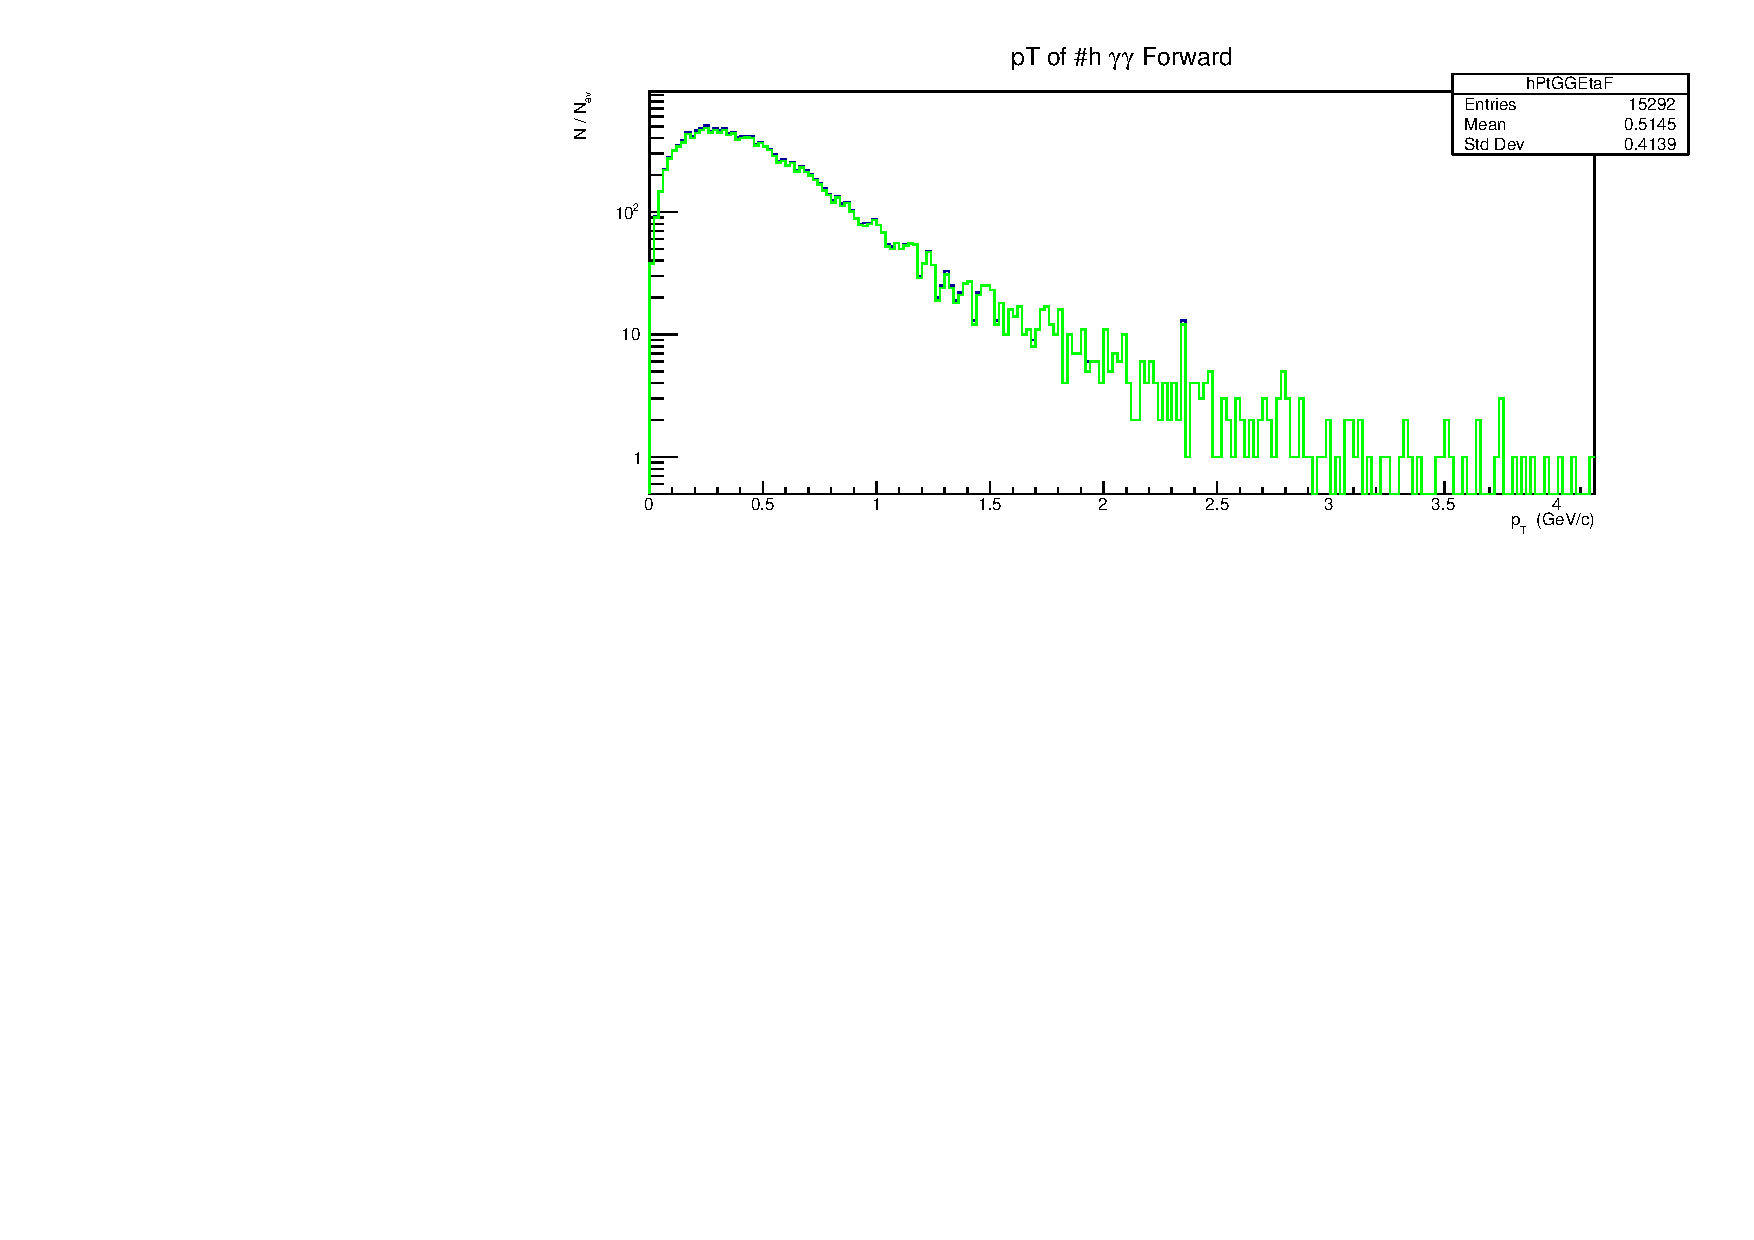
\includegraphics[width=0.32\textwidth]{/Users/marin/alice3/alice3Conversions//anaConv/EtaMeson-EtaMesonCut-Forward.pdf}&
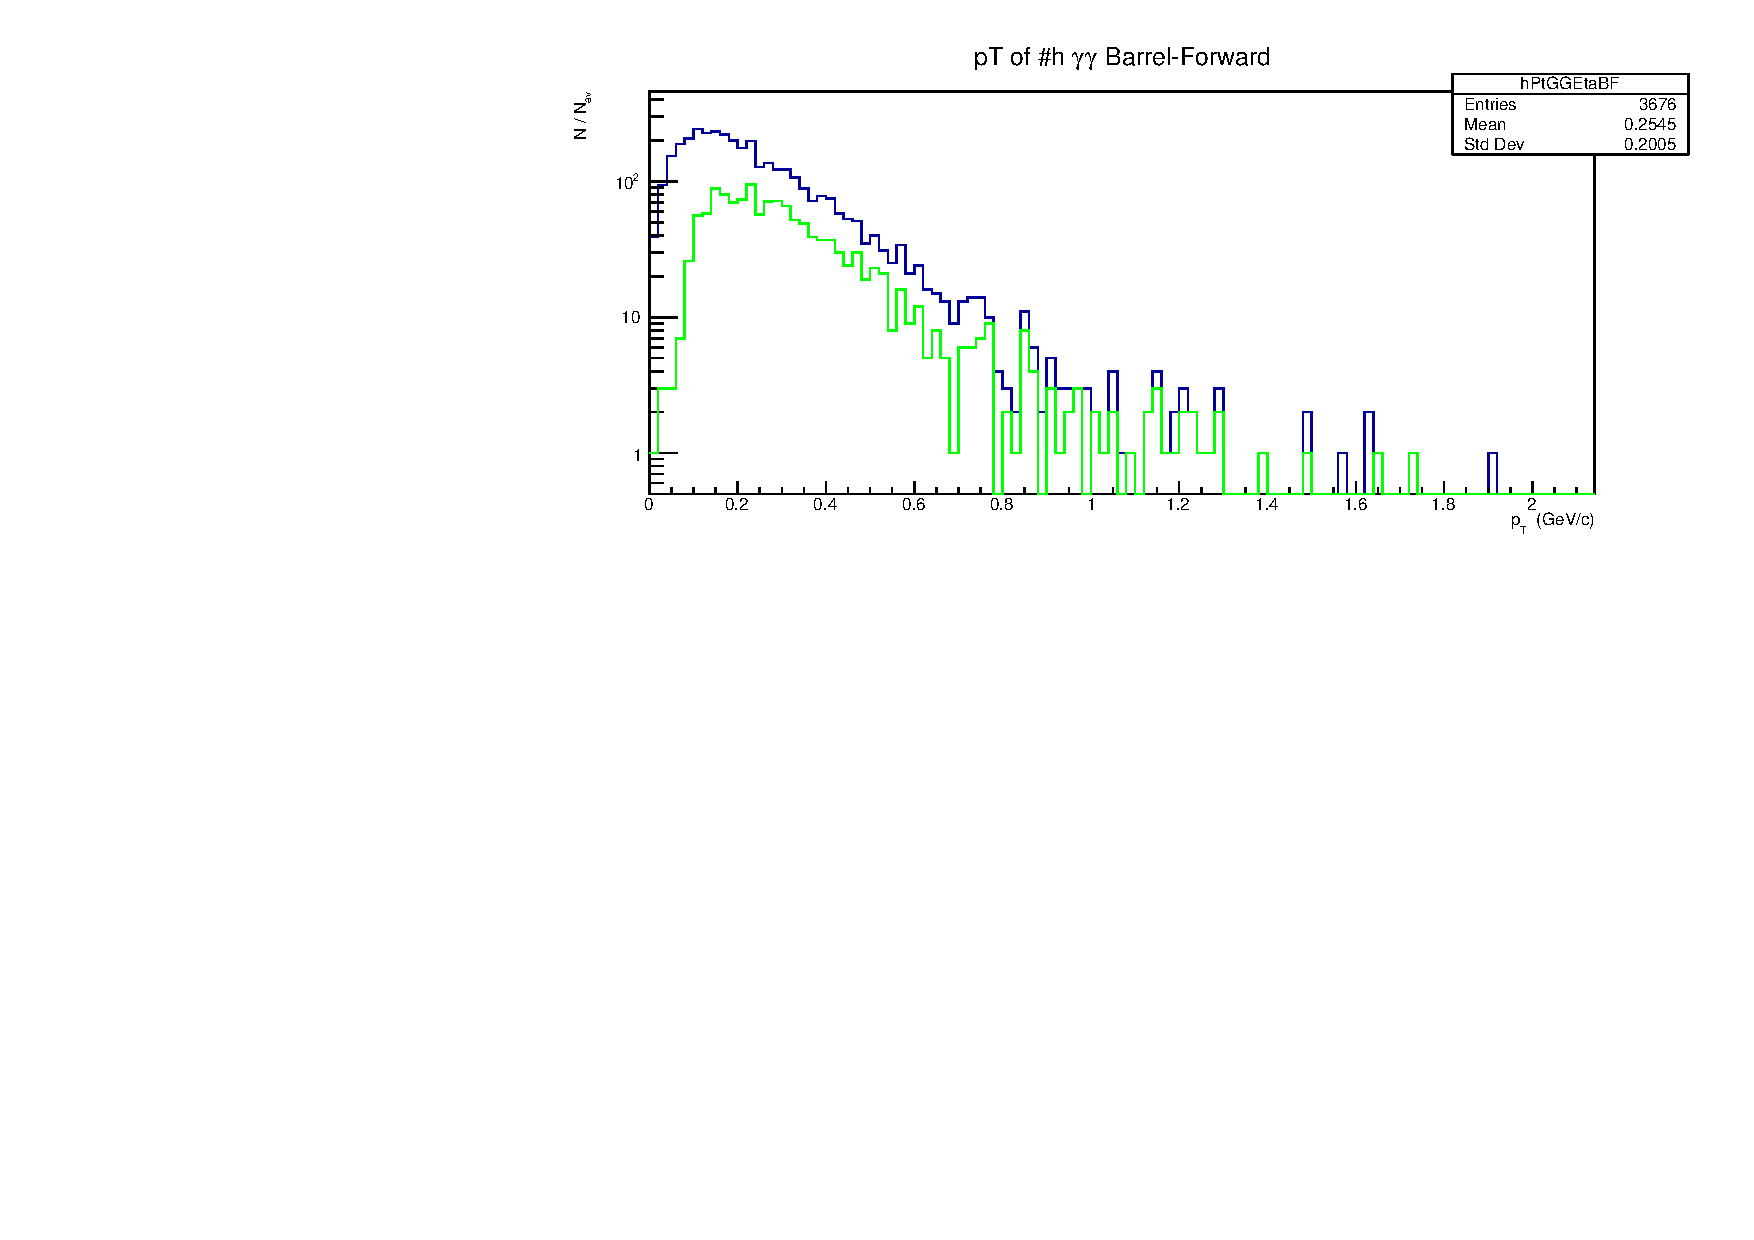
\includegraphics[width=0.32\textwidth]{/Users/marin/alice3/alice3Conversions//anaConv/EtaMeson-EtaMesonCut-Barrel-Forward.pdf}\\
Barrel & Forward & Barrel-Forward \\
\end{tabular}


\end{frame}


\end{document}




